\documentclass[papersize]{suribtabst}

% 必要なパッケージ又はマクロはこの辺りに定義
% 下記はサンプルで,常に読み込まねばならないわけではない.
\usepackage{graphicx}
\usepackage{amsmath}
\usepackage{amssymb}
\usepackage{amsthm}
\usepackage{amsfonts}
\usepackage{latexsym}
\usepackage{breakcites}
\usepackage{float}

% 論文タイトル:日本語だけの場合
\title{特許検索における質問意図の曖昧化}
% 論文タイトル:英語の場合は日本語タイトルを併記
%\title{Writing a Master's Thesis in Mathematical Engineering Department\\ \vspace{0.4em}(数理情報学専攻における修論執筆に関する研究)}
 
%\titlewidth{}% タイトル幅 (指定するときは単位つきで)
\author{胡 瀚林}
\eauthor{HANLIN HU}% Copyright 表示で使われる
\studentid{48-156229}
\supervisor{中川 裕志 教授}% 1 つ引数をとる (役職まで含めて書く)
%\supervisor{指導教員名 役職 \and 指導教員名 役職}% 複数教員の場合,\and でつなげる
\handin{2017}{1}% 提出月. 2 つ (年, 月) 引数をとる

% 本文ここから

\begin{document}
\maketitle

\section{はじめに} % セクション名等は適宜付け替えること
企業が特許を取る前に,類似な特許が既に存在するかを確かめるために特許データベースを検索する必要がある.
テキスト検索をするとき,検索質問をサーバ側に渡さなければならない.
しかし,検索質問から質問者の情報が漏洩する危険があることがAOL事件\cite{AOL}より証明された.
特許検索の場合は検索質問が研究開発動向など企業秘密を含んでいるため,一般的なウェブ検索の質問者より質問のプライバシー問題を重視している.
ウェブテキスト検索の質問から質問者の検索意図を守る手法が多数存在している.
その中では真の質問と同時にダミー質問を提出する質問曖昧化手法が一番効率的,現実的である.
本論文では特許検索における既存の質問曖昧化手法を実装し,
類似度攻撃\cite{simattack2016}で特許データベースにおける既存手法の安全性を評価した.
また,類似度攻撃を含め,多くの既存の質問曖昧化に対する攻撃手法は攻撃者が質問者に関する事前情報を持つと仮定する.
本論文では事前情報なしの攻撃手法を提案し,その攻撃手法に対応する既存の質問曖昧化の改良と新たな質問曖昧化手法を提案し,
特許データベースにおける評価実験を行う.

\section{特許の概要}
特許文書は発明を正確に規定するために普段に使わない学術用語を用い,単語を全体を通じて統一して使用して単語を曖昧性を無くす.

また特許文書は世界標準である国際特許分類コードが付いている.
国際特許分類は階層構造であり,一番上の階層はAからHまでの8個のセクションである.

特許検索の質問は一般なウェブ検索質問より長い.

\section{既存研究}
\subsection{曖昧化手法}
事前に質問をグループにする手法(PDS)\cite{providing2009}:
否認可能検索は
文書集合から高頻度な単語と単語ペアをシード質問として抽出し,
潜在意味分析(LSA)\cite{LSA1990}を用いてシード質問をトピック空間にマップし,
トピック空間に距離が近いシード質問をクラスタリングして標準質問にし,
トピック空間に距離が遠い標準質問でPD-質問集合を構築する.
検索する場合は,質問者が検索したい質問の代わりに
事前に用意した標準質問集合からトピック空間において質問者が検索したい真の質問と最も近い標準質問が属するPD-質問集合をサーバに提出し,
サーバから検索結果を得,質問者側で真の質問を用いて検索結果をフィルタリングする.

事前に単語をグループにする手法(ETSQ)\cite{embellishing2010}:
質問者のプライバシーを保護する質問加工法は
単語を類義関係のセット(synset)でグループ化するWordNet\cite{wordnet1995}を用いて意味的に遠い単語を1つ単語バケットにし,
真の質問単語が属するバケットの中の他の単語を全てダミー単語として質問に加え,
1つの加工した質問として検索サーパに提出する.
暗号したままの暗号文を加算できる加算可能な準同型暗号\cite{dpe1994}を用いることにより真の質問の単語だけ検索することができる.

事前にトピックをグループにする手法(HDGA)\cite{masking2014}:
質問意図を曖昧化するキーワード検索は
潜在的ディリクレ配分法(LDA)\cite{lda2003}を用いてコーパスにおける
各トピック$t$における単語$w$の出現率$Pr(w|t)$を計算する.
検索する場合は
ハッシュ関数HRW\cite{hrw1998}を用いてダミートピック$t'$を選び,
$Pr[w|t']$に基づいて単語をランダムに選び,真の質問と同じ長さのダミー質問を作る.

\subsection{攻撃手法}
事前情報がある場合の類似攻撃(SimAtt)\cite{simattack2016}:
SimAttは質問者が提出した質問と攻撃者が事前に得た質問者の質問ログ間の類似度を計算し,
同じ質問グループの中の質問ログとの類似度が一番高い質問を真の質問とする.

\section{本研究で提案するアルゴリズム}
\subsection{攻撃手法}
メイントピック攻撃(MTA):
ダミー質問が真の質問と同様に全ての単語が1つのトピックに集中することが失敗したら,
真の質問と真の質問のメイントピックの関連値がダミー質問とダミー質問のメイントピックの関連値より強いと考えられる.
MTAは1つの質問グループの中で自分のメイントピックとの関連値が一番高い質問を真の質問とする.

事前情報がない場合の類似度攻撃(SimAtt2):
攻撃者が事前的に質問者の真の質問ログを持たないとSimAttを用いることができない.
SimAtt2は意味的に近い一連の質問が真の質問の列であると考える.
SimAtt2は1つの質問グループに属する質問と同じ数の質問列を可能な真の質問列として保存し,
次にきた質問グループの各質問に対して各可能な真の質問列との類似度を計算し,一番類似度が高い質問列に加える.
類似度が一番高い質問と質問列のペアを真の質問の列とする.

\subsection{単語ベクトルを用いた質問曖昧化}

全ての単語を単語とトピック$t$の関連値を大きい順に並べるベクトルをトピック$t$の単語ベクトルという.

質問者が検索したいトピックを曖昧化する質問曖昧化(QOT):
\begin{figure}[H]
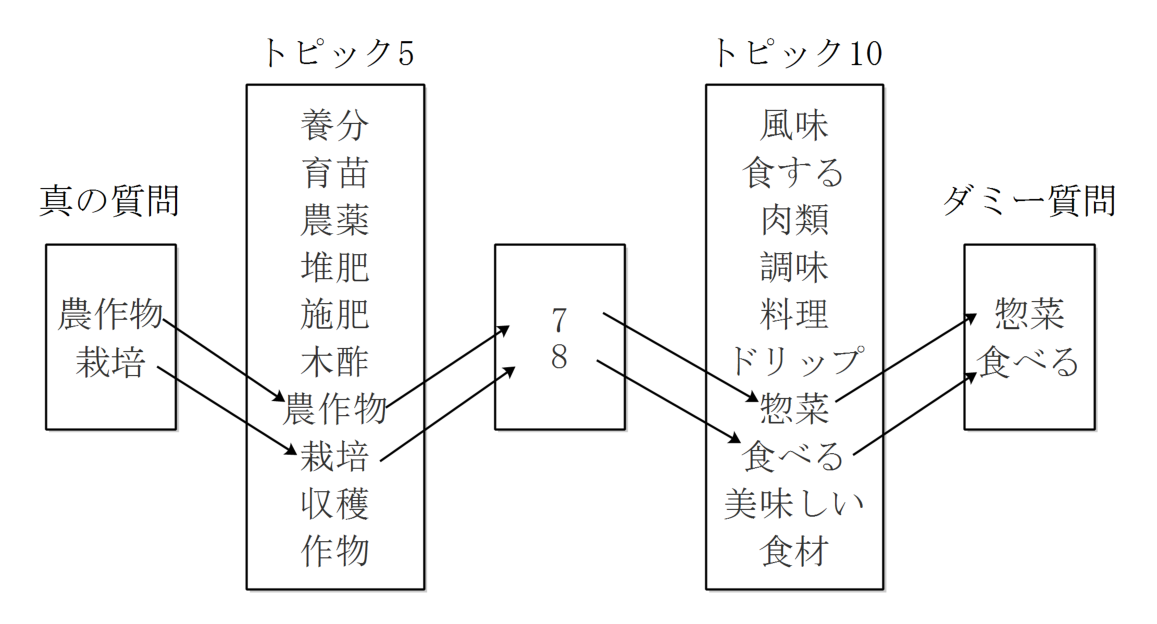
\includegraphics[width=0.2\textwidth,natwidth=195.813,natheight=105.625]{QOT.pdf}
\end{figure}






% 文献リスト:

\bibliographystyle{apalike}%           BibTeX を使う場合
\bibliography{thesis}% BibTeX を使う場合

%\begin{thebibliography}{99} % 普通に \bibitem を埋め込む場合
%\end{thebibliography}


\end{document}